\documentclass[12pt, letterpaper]{article}

\usepackage{graphicx} % Graphics
\usepackage{amsmath, amsfonts, amssymb, amsthm} % Math stuff
\usepackage{enumerate, array, multirow}

\usepackage{caption}
\usepackage{subcaption}
\usepackage{color}
\newcommand{\hilight}[1]{\colorbox{yellow}{#1}}
%%%  Language Settings  %%%

%\usepackage[spanish]{babel}  % Spanish language
% \usepackage[applemac]{inputenc}  % Allows for accents!! Useful for spanish documents
%\usepackage[latin1]{inputenc}


%%%  Page settings  %%%
%\usepackage{fullpage} % quick-and-dirty way to get 1in for all margins
\usepackage[left=2cm,top=2cm,right=2cm,bottom=2.5cm,nohead]{geometry}

\title{Resonancia en bah\'ias utilizando el m\'etodo de elementos finitos}
\author{Jos\'e Galaz, Jaime Soto}
\date{}

\begin{document}
\maketitle

\begin{abstract}
    A menudo la propagaci\'on y superposici\'on de ondas en bah\'ias origina oscilaciones de per\'iodos largos que ocasionan inundaci\'on y da\~no inesperado en embarcaciones y estructuras, sin embargo, a partir de las ecuaciones de Navier-Stokes es posible deducir que, cuando estas ondas largas poseen peque\~na amplitud, las frecuencias y modos de oscilaci\'on corresponden a los valores y vectores propios dados por la ecuaci\'on de Helmholtz. En este trabajo ha sido posible desarrollar una formulaci\'on variacional del problema, e implementar computacionalmente el m\'etodo de Galerkin para calcular los modos de resonancia aproximados para una bah\'ia de geometr\'ia arbitraria. Ha sido posible validar con soluciones anal\'iticas y se ha aplicado el m\'etodo para estudiar la bah\'ia de Concepci\'on, Chile, encontrando que los per\'iodos de oscilaci\'on son de orden de magnitud esperado, y similares a los de un tsunami, y que la forma de los modos principales concuerda con lo que se reporta en la literatura \cite{Belloti2012}.
\end{abstract}

\section{Introducci\'on}

El fen\'omeno de resonancia al interior de una regi\'on  semicerrada reviste una especial importancia en el estudio del comportamiento de ondas que se propagan desde el oc\'eano hacia zonas costeras y que puede inducir la amplificaci\'on de \'estas al ingresar a una regi\'on semicerrada \cite{Kowalik1993}. El fen\'omeno de resonancia puede condicionar el dise\~no de puertos y comportamiento de naves al interior de estos \cite{Diaz2006web}, la inundaci\'on por efecto de tormentas y marejadas \cite{Kowalik1993} y en la amplificaci\'on y/o aparici\'on de ondas de tsunami tard\'ia, horas despu\'es de la llegada de la primera onda \cite{Kowalik1993}. Esta \'ultima podr\'ia ser una explicaci\'on para describir las caracter\'isticas que tuvo el tsunami de Maule 2010 \cite{Cyper2012web}.

Existen varias formas de aproximarse a una identificaci\'on y cuantificaci\'on de los modos propios de oscilaci\'on al interior de una bah\'ia. Una de \'estas es propagar varias ondas (distinta frecuencia y direcci\'on) hacia el interior y cuantificar la amplificaci\'on de estas. Esta propagaci\'on puede ser lineal o no lineal \cite{Mei2005}. Otra aproximaci\'on consiste en calcular directamente los modos propios de oscilaci\'on de la ba\'hia \cite{Belloti2012, Mei2005}. Esta \'ultima aproximaci\'on es la utilizada en este trabajo.

El objetivo de este trabajo es implementar un software computacional que permita determinar los modos de oscilaci\'on de una bah\'ia de geometr\'ia arbitraria utilizando una aproximaci\'on por elementos finitos. La mayor dificultad que presenta una aproximaci\'on directa para la determinaci\'on de los modos propios es la de seleccionar una condici\'on de borde apropiada a cada caso \cite{Mei2005, Rabino2009}. Como una primera aproximaci\'on se considerar\'a una bah\'ia cerrada.

Para encontrar una aproximaci\'on a los modos propios se resuelve la ecuaci\'on de Helmholtz mediante el m\'etodo de elementos finitos, aplicado a una bah\'ia cerrada con condiciones de borde Neumman $u,_i  n_i = 0$. La ecuaci\'on de Helmholtz es deducida de las ecuaciones de Navier-Stokes y presentada en su formulaci\'on fuerte. Se obtiene la formulaci\'on variacional y de Galerkin asociada al problema fuerte y se implementan elementos tipo \verb;tri3; para la resolucion de la ecuacion matricial. El modelo es validado en una geometr\'ia rectangular cuya soluci\'on anal\'itica es conocida y aplicado al caso real de la Bah\'ia de Talcahuano


\section{Marco Te\'orico}
  \subsection{Ecuaciones fundamentales}
  \label{subsec:ecuaciones}
  Sea  $\Omega' \subset \mathbb{R}^3$ el dominio de inter\'es, $t_f>0$ el tiempo final de la simulaci\'on,   $\vec v : [0,t_f]\times \Omega' \rightarrow  \mathbb{R}^3$ el campo de velocidad, y $p : [0,t_f] \times \Omega' \rightarrow \mathbb{R}$ el campo de presiones, de un fluido incompresible con densidad $\rho \in \mathbb{R}^+$, que escurre sobre un fondo (topograf\'ia - batimetr\'ia) de forma dada por $b:\Omega' \rightarrow \mathbb{R}$. Si se desprecian efectos disipativos y se consideran fuerzas de volumen $\vec f_b = (0,0,-g)^T$, con $g$ la aceleraci\'on de gravedad, las ecuaciones de Navier-Stokes son \cite{toro}
\begin{align}
  \begin{split}
    \nabla \cdot \vec v &= 0 \\
    \frac{\partial }{\partial t}\vec v + \nabla \cdot \vec v \otimes \vec v  &= -\frac{1}{\rho}\nabla p + \vec f_b    \\
    v_3|_{z=\eta	} &= \frac{\partial \eta}{\partial t}+(\vec v \cdot \nabla )\eta \\
    v_3|_{z=b} &= \frac{\partial b}{\partial t} + (\vec v \cdot \nabla )b \\    
    p|_{z = \eta} &= 0
  \end{split}  
  \label{NS-incompresible}
\end{align}

En particular, en una bah\'ia de interior $\Omega \subset \mathbb{R}^2$, con borde impermeable $\partial\Omega_h$ y linea nodal $\partial \Omega_g$ tales que $\partial \Omega = \partial \Omega_h \cup \partial \Omega_g$ , y bajo el supuesto que las ondas son suficietemente largas, de forma que las aceleraciones verticales no tienen influencia significtiva sobre el perfil de presiones hidrost\'atico, y por medio de integraci\'on vertical entre el fondo $b$ y la superficie libre $\eta$, las Ecuaciones No Lineales de Aguas Someras (Non-Linear Shallow water Equations, NSWE) son, 

\begin{align}  \begin{split}
\frac{\partial}{\partial t}\left(\eta\right)+\frac{\partial}{\partial x}\left(hu\right)+\frac{\partial}{\partial y}\left(hv\right) & =0  \text{       si } x \in \Omega\\
  \frac{\partial}{\partial t}\left(hu\right)+\frac{\partial}{\partial x}(hu^{2}+\frac{1}{2}gh^{2})+\frac{\partial}{\partial y}(huv) & =-gh\frac{\partial}{\partial x}b  \text{   si } x\in\Omega\\
  \frac{\partial}{\partial t}\left(hu\right)+\frac{\partial}{\partial x}(huv)+\frac{\partial}{\partial y}(hv^{2}+\frac{1}{2}gh^{2}) & =-gh\frac{\partial}{\partial y}b  \text{     si } x \in \Omega\\
  (hu,hv) \cdot \vec n &= 0  \text{ si    } x\in\partial \Omega_h \\
   \eta &= 0  \text{ si    } x \in \partial \Omega_g  
  \end{split}
  \label{eq:nswe_cart}
  \end{align}
donde, viendo la figura \ref{fig:vars}, $h:(t,x,y) \in [0,t_f] \times \Omega \to \eta(t,x,y)-b(x,y) \in \mathbb{R}^+$ es la altura de la columna de agua,  y $(u,v)$ las componentes de velocidad horizontal promediadas en la vertical, dadas por
 $$
  (u,v)=\frac{1}{h}\int_{b}^\eta (v_1,v_2)dz
 $$
  
  \begin{figure}
    \centering
    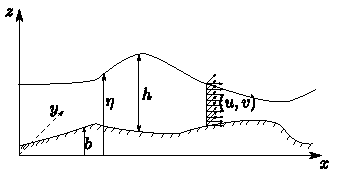
\includegraphics[width=10cm]{figs/variables.pdf}    
    \caption{ Vist esquem\'tica de ls varibles hidrodin\'amicas definidas para las Ecuaciones No Lineales de Aguas Somers (NSWE).}
    \label{fig:vars}
  \end{figure}

Las ecuaciones en \eqref{eq:nswe_cart}, forman un sistema hiperb\'olico de ecuaciones diferenciales parciales no lineales, que admite ondas de choque e interfaces seco-mojado, cuando $h$ tiende a $0$. Sin embargo, es posible obtener una linealizaci\'on del sistema \eqref{eq:nswe_cart} si se consideran peque\~nas perturbaciones a una masa de agua en reposo, es decir si
$$
	\eta=h_0+\eta' \hspace{.5cm} u=0+u',\hspace{.5cm} v = 0 + v'
$$
donde la notaci\'on $\square'$ indica peque\~nas perturbaciones sobre $\square$, y $h_0:\Omega\rightarrow \mathbb{R}$ representa la altura de la columna de agua, de forma que  \footnote{Aqu\'i el lector debe notar que este supuesto es equivalente a asumir que las ondas son de amplitud peque\~na.}
$$\left|\frac{\eta'(t,x,y)}{h_0(x,y)}\right|<<1$$
para cualquier $(t,x,y) \in [0,t_f]\times\Omega$. Bajo estos supuestos, se deducen las Ecuaciones Lineales de Aguas Someras (LSWE), dadas por
\begin{align}
	\begin{split}
	\frac{\partial \eta'}{\partial t}+\frac{\partial h_0u'}{\partial x}+\frac{\partial h_0v'}{\partial y} = 0  \text{ si } x \in \Omega\\
    \frac{\partial u'}{\partial t} + g\frac{\partial \eta'}{\partial x}=0  \text{ si } x \in \Omega\\
    \frac{\partial v'}{\partial t} + g\frac{\partial \eta'}{\partial y} = 0  \text{ si } x \in \Omega \\
    (h_0u',h_0v') \cdot \vec n = 0 & \text{ si } x\in\partial \Omega_h \\
   \eta' = 0  \text{ si } x \in \partial \Omega_g  
    \end{split}
    \label{swe}
\end{align}

    Si ademas $\eta',u',v' \in \mathcal{C}^2(\Omega)$, multiplicando la segunda y tercera ecuaci\'on de \eqref{swe}, por $h$ y derivando respecto a $x$ e $y$ es cierto que 
    \begin{equation}
    	\begin{split}
    	\frac{\partial^2 \eta}{\partial t^2} - \nabla \cdot( gh \nabla \eta) = 0, \text{ si } x \in \Omega \\
        \frac{\partial \eta}{\partial \vec n} = 0 \text{ si } x \in \partial \Omega_h \\
        \eta = 0 \text{ si }x \in \partial \Omega_g
        \end{split}
     \label{eqonda}
    \end{equation}

    donde se cambi\'o de notaci\'on al usar $\square$ como $\square'$. Las ecuaciones \eqref{eqonda} corresponden a la ecuaci\'on lineal de onda,  de celeridad $c=\sqrt{gh}$, revelando la similitud entre la propagaci\'on de ondas de amplitud peque\~na en una bah\'ia, con la de ondas ac\'usticas o el\'asticas lineales.
    
    Finalmente, si se estudian ondas estacionarias, es posible separar variables y escribir (abusando de notaci\'on en $u$), con $u:\Omega \rightarrow \mathbb{R}$
    \begin{equation}
    	\eta(t,x,y) =Re\left\{ u(x,y) e^{-i \omega t}\right\}
    \end{equation}
    
    lo cual, sustituyendo en \eqref{eqonda}, conduce a 
    
    \begin{equation}
      \begin{split}
    	\nabla \cdot \left( gh_0 \nabla u\right) + \omega^2 u = 0 \text{ si } x \in \Omega\\
        \frac{\partial u}{\partial \vec n} = 0 \text{ si } x \in \partial \Omega_h \\
        u = 0 \text{ si } x \in \partial \Omega_g
      \end{split}
        \label{helmholtz}
    \end{equation}
    
    El sistema \eqref{helmholtz} es m\'as conocido como la Ecuaci\'on de Helmholtz, y denota un problema de valores y vectores propios del operador diferencial de la ecuaci\'on de Poisson ($\nabla \cdot c^2 \nabla \square$). Es posible demostrar \cite{nica2011}, que la extensi\'on d\'ebil del operador de Poisson definido sobre $L^2(\Omega,\mathbb{R})$ posee una cantidad numerable de valores y vectores propios $(\lambda_n, u_n)_{n\in\mathbb{N}}$, tales que $u_n\neq 0$ y $0\leq \lambda_1$ y $\lambda_n \leq \lambda_{n+1}$. Adem\'as es f\'acil verificar, que para el caso en que $ \partial \Omega _g = \varnothing$, como es el caso de una bah\'ia cerrada, si $u(x,y)=K \in \mathbb{R}$ para cualquier $(x,y)\in\Omega$, entonces \eqref{helmholtz} se satisface trivialmente y $\lambda=0$ es el primer valor propio, lo cual corresponde f\'sicamente a cuando la superficie libre del agua est\'a a un nivel constante, es decir, cuando la masa de agua est\'a en reposo. Lo anterior se debe tener en consideraci\'on al examinar los valores propios obtenidos num\'ericamente.
    %f\'isicamente, como $T=2\pi/\sqrt{\lambda}=\infty$ y $u=K$, indica que el primer modo de vibraci\'on de la bah\'ia corresponde uniformes de la superficie libre $\eta$, en todo el dominio.
%     
%     @article{nica,
% 	title="Eigenvalues and Eigenfunctions of the Laplacian",
% 	author="Mihai Nica",
% 	journal="The Waterloo Mathematics Review",
% 	year="2011",
% 	volume=1,
% 	number=2,
% 	pages={23--34},
% }
    
    
  \subsection{Formulaci\'on variacional y de Galerkin}
  La formulación fuerte del problema de valor de frontera es: (ecuaci\'on \eqref{helmholtz}

\begin{align*}
\text{Dados $g$, $h: \Omega \rightarrow \mathbb{R}$, encontrar $(u, \omega^2)$ tal que:}\\
\omega^2 u + (gh u,_i),_i  = 0, \ \ \ \ & \boldsymbol{x} \in \Omega \\
\frac{\partial u}{\partial n} = u,_i n_i = 0, \ \ \ \ & \boldsymbol{x} \in \partial \Omega_h \ & (S) \\
u=0, \ \ \ \ &\boldsymbol{x} \in \partial \Omega_g\\
\end{align*}

Sean:\\ \\
$ \mathcal{V} = \left \{ v \in H^1 (\Omega, \mathbb{R}) \ /\  v|_{\partial \Omega_g} = 0 \right \}$\\
$ \mathcal{S} = \left \{ u \in H^1 (\Omega) \ /\  u,_i n_i = 0, \ \ \boldsymbol{x} \in \partial \Omega_h \right \}$\\ 

multiplicando la ecuaci\'on de Helmholtz por $-v \in \mathcal{V}$ e integrando por partes:\\

$$-\int_{\Omega} v \left( \omega^2 u + (gh u,_i),_i \right) \mathrm{d}\boldsymbol{x} = 0$$

$$-\int_{\Omega} v ( \omega^2 u )\mathrm{d}\boldsymbol{x} -\int_{\partial \Omega} v (gh u,_i) n_i \mathrm{d} S
+\int_{\Omega} v,_i g h u,_i \mathrm{d}\boldsymbol{x} = 0$$

Pero, por condici\'on de borde: $u,_i n_i = 0 \ \forall \boldsymbol{x} \in \partial \Omega_h$, luego

$$-\int_{\Omega} v ( \omega^2 u )\mathrm{d}\boldsymbol{x} 
+\int_{\Omega} v,_i g h u,_i \mathrm{d}\boldsymbol{x} = 0$$

O, en forma abstracta:
\begin{equation}
a(v, u) - \omega^2 (v, u) = 0
\label{eq:debil_abstracta}
\end{equation}

Luego, 

\begin{align*}
\text{Dados $g$, $h: \Omega \rightarrow \mathbb{R}$, encontrar $(u, \omega^2)$, $u \in \mathcal{S} $, $\omega \in \mathbb{R}$, tal que:}\\
a(v, u) - \omega^2 (v, u) = 0 \ \ \ \ \  & (W) \\
\end{align*}

Formulaci\'on Galerkin:

Sean $u^h \in \mathcal{S}^h \left(\equiv \mathcal{V}^h \right)$ con $\mathcal{V}^h \in \mathcal{V}$

entonces:

$$ a(v^h, u^h) - \omega^2 (v^h, u^h) = 0 $$

Luego la formulaci\'on galerkin queda:




\section{Resultados}
   \subsection{Bah\'ia rectangular de ancho unitario}
  Para validar los resultados de la implementaci\'on del algoritmo, y estudiar la convergencia de \'este, se ha escogido una soluci\'on anl\'itica al problema presentado en la ecuaci\'on \eqref{helmholtz}. Este caso corresponde a una bah\'ia cuadrada de largo unitario cuyo interior es $\Omega = [0,1]\times[0,1]$, la cual se encuentra cerrada por bordes impermeables, es decir, $\partial \Omega_g=0$, y fondo a profundidd $h_0\in\mathbb{R^+}$. Por medio de separaci\'on de variables, al asumir que $u$ puede escribirse como $u(x,y)=f(x)g(y)$, y al considerar las condiciones de borde, se deduce que los modos de oscilaci\'on vienen dados por 
  
  \begin{equation}
    \begin{array}{cc}
    u_{nm}(x,y)=A_{nm}\cos(n\pi x)\cos(m\pi y) & \text{ con } n,m \in \mathbb{N}_0 \text{ y } A_{nm}\in\mathbb{R}
    \end{array}
    \label{eq:bahia_cerrada_modo}
  \end{equation}

  y el per\'iodo de oscilaci\'on asociado
  
  \begin{equation}
    \begin{array}{cc}
    T_{nm}=\dfrac{2}{\sqrt{gh}}\left( n^2+m^2\right)^{-1/2} & \text{ con } n,m \in \mathbb{N}_0
    \end{array}
    \label{eq:bahia_cerrada_periodo}
  \end{equation}

La soluci\'on mediante FEM es implementada para distintas resoluciones de malla y analizada su convergencia mediante la determinaci\'on del error asociado al valor propio y el error asociado al vector propio correspondiente.

Para el caso del error en el valor propio se utilza norma natural de $\mathbb{R}$

$$E = |\lambda^h - \lambda|$$

donde  \hilight{$\lambda$} es la longitud de onda obtenida mediante la soluci\'on anal\'itica \hilight{$\lambda^h$} es la longitud de onda obtenida mediante aproximaci\'on por FEM\\

Para el caso del error en el valor de la desnivelaci\'on superficial el error se calcula mediante la norma de $\mathcal{L}^2(\Omega,\mathbb{R})$

$$E = \left(\int_{\Omega} (u^h - u) \mathrm{d}\boldsymbol{x} \right)^{1/2}$$

Los resultados para el valor propio se muestran en la figura \ref{fig:velores_propios}

\begin{figure}
  \centering
  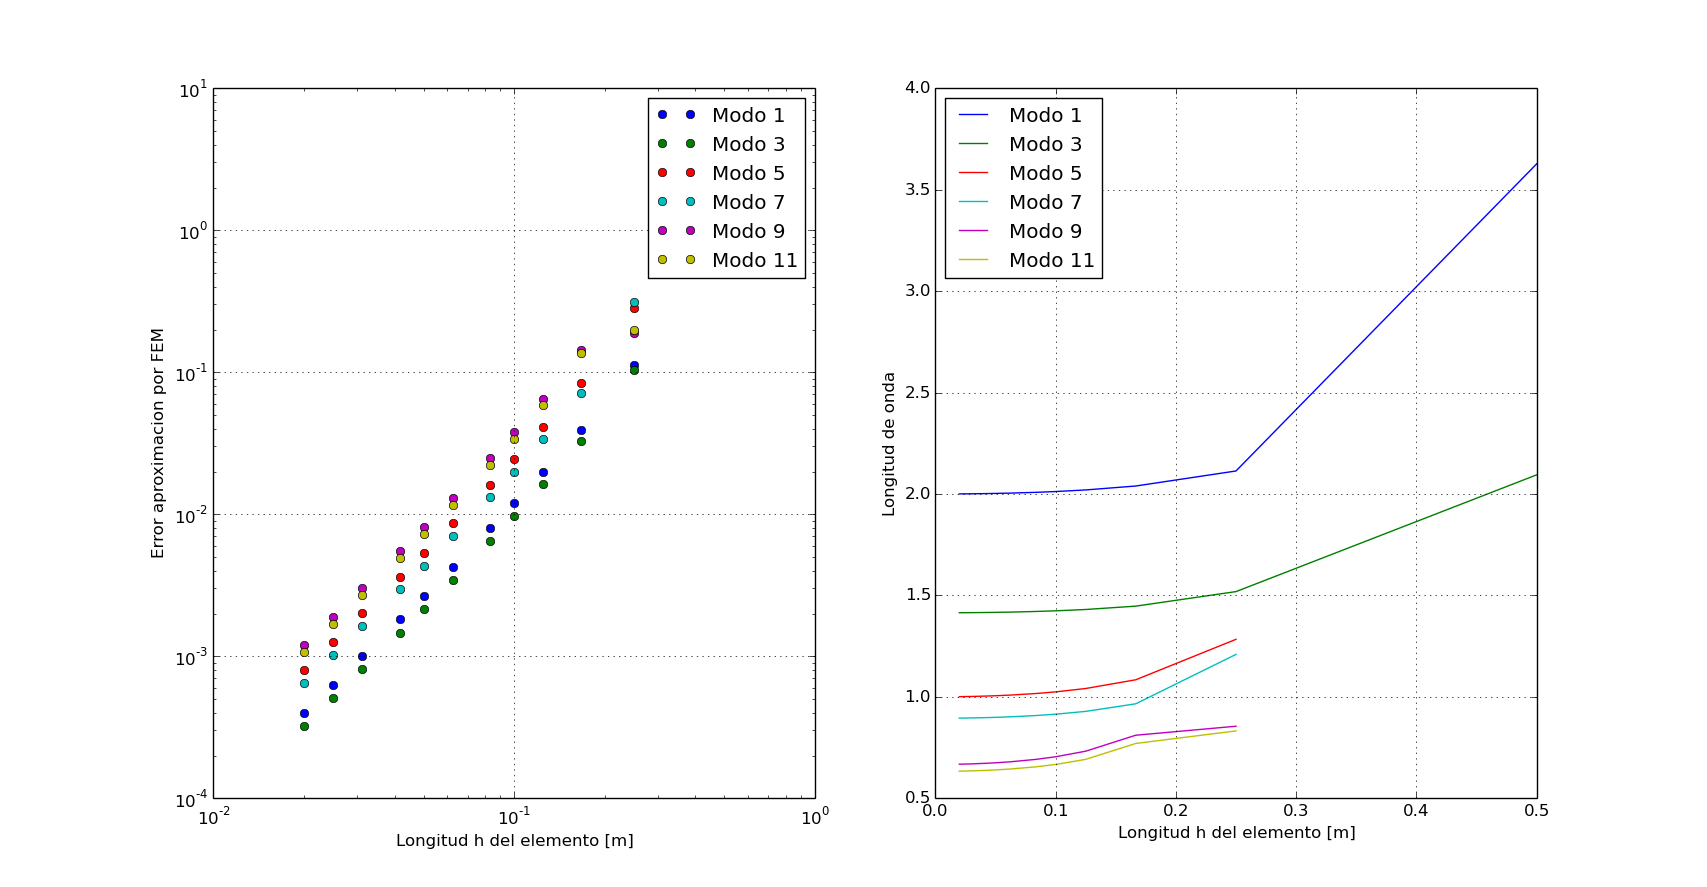
\includegraphics[width=17cm]{figuras/valores_propiosFEM.png}
  \caption{ Resultados aproximaci\'on valores propios mediante FEM y errores asociados}  
  \label{fig:velores_propios}
\end{figure}

Ajustando una curva a los datos ($log(E)$, $log(h)$) se obtiene una recta $log(E) = log(C) + p log(h)$ donde p es la taza de convergencia


\begin{table}[h]
\centering
\begin{tabular}{|c|c|c|}
\hline 
Modo & C & p \\ 
\hline 
1 & 0.62007961 & 2.4403783 \\
\hline 
3 & 0.39830035 & 2.33894099 \\ 
\hline 
5 & 0.69813644 & 2.26494859 \\  
\hline 
7 & 0.71017628 & 2.33846474 \\ 
\hline 
9 & 0.68486822 & 2.12311422 \\  
\hline 
11 &  0.70325574 & 2.17136287 \\
\hline 
\end{tabular} 
\caption{\hilight{Coeficientes de ajuste de las curvas $\log(E_\lambda)=\log(C)+p\log(h)$}}
\end{table}

Para el caso de la convergencia de los \hilight{vectores propios}, los resultados se muestran en la figura \ref{fig:vectores_propios}

\begin{figure}
  \centering
  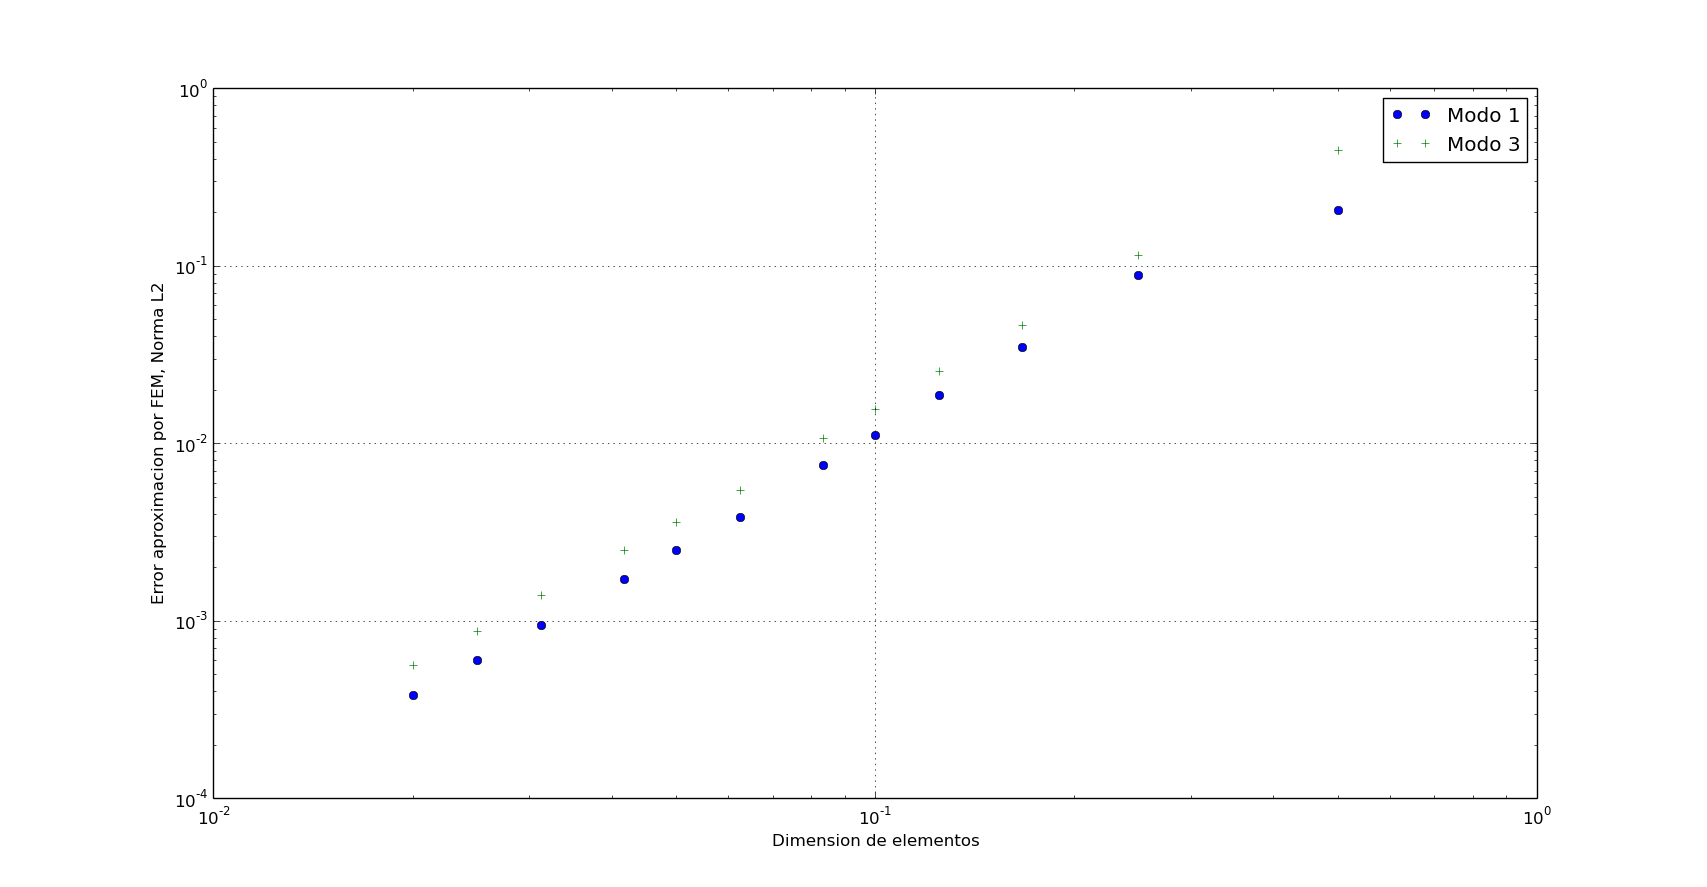
\includegraphics[width=17cm]{figuras/vectores_propiosFEM.png}
  \caption{ \hilight{Errores en norma $\mathcal{L}^2$ de los vectores asociados a cada modo propio}  }
  \label{fig:vectores_propios}
\end{figure}

Ajustando una recta a los datos ($log(E)$, $log(h)$)
\begin{table}[h]
  \centering
  \begin{tabular}{|c|c|c|}
  \hline 
  Modo & C & p \\ 
  \hline 
  1 & 0.0765871 & 2.04894336 \\  
  \hline 
  3 & 0.29036431 & 2.09300275 \\  
  \hline 
  \end{tabular} 
  \caption{\hilight{Coeficientes de ajuste de las curvas $\log(E_u)=\log(C)+p\log(h)$}}
\end{table}

En ambos casos se puede ver que la taza de convergencia es de orden 2.

\begin{figure}
  \centering
  \begin{subfigure}{0.3\textwidth}
    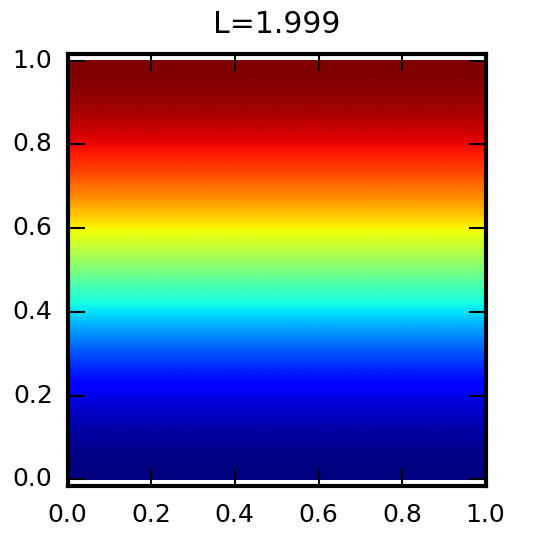
\includegraphics{figuras/modonum_1.png}
  \end{subfigure}
  ~
  \begin{subfigure}{0.3\textwidth}
    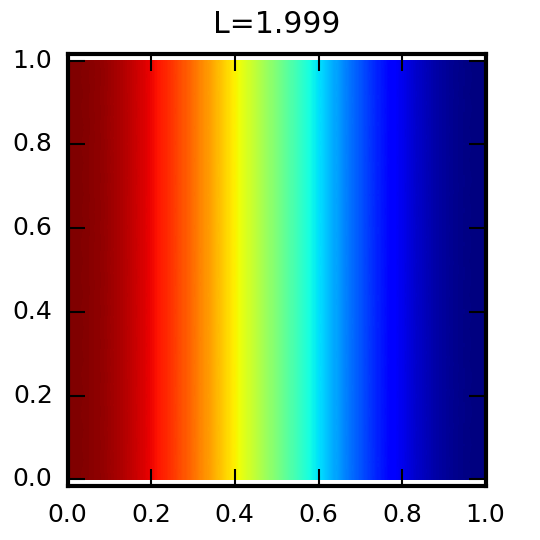
\includegraphics{figuras/modonum_2.png}
  \end{subfigure}
  
  \caption{Ejemplo de la multiplicidad de valores propios: modos de oscilaci\'on 1 y 2 usando $h=1/25$  mediante el m\'etodo de Elementos Finitos.}
\end{figure}

\begin{figure}  
  \centering
  \begin{subfigure}{0.4\textwidth}
    \centering
    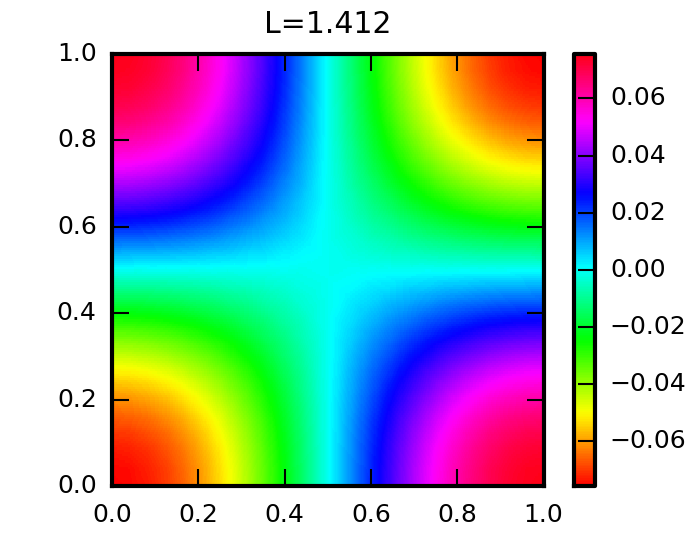
\includegraphics{figuras/modonum_3.png}
  \end{subfigure}
  ~
  \begin{subfigure}{0.4\textwidth}
    \centering
    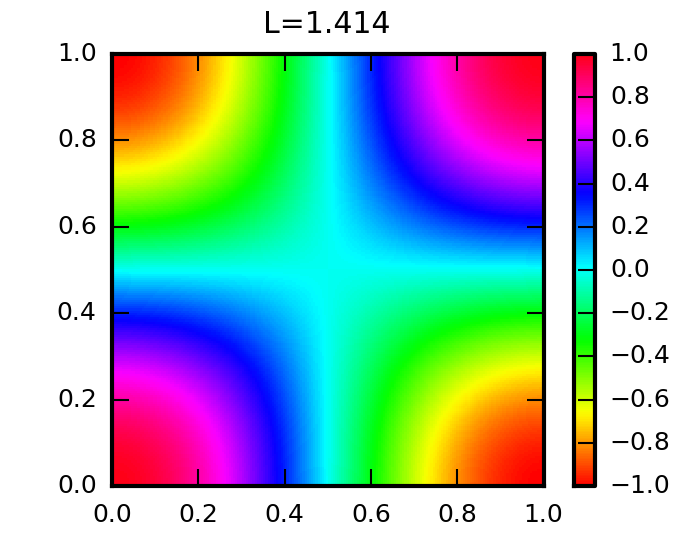
\includegraphics{figuras/modoanalitico_1_1.png}
  \end{subfigure}
  
  
  \begin{subfigure}{0.4\textwidth}
    \centering
    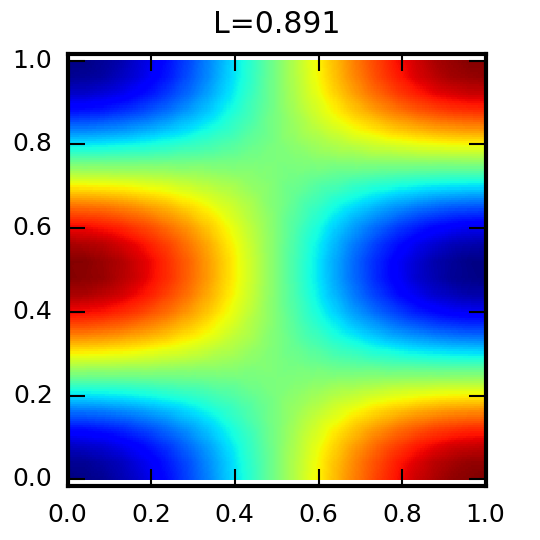
\includegraphics{figuras/modonum_6.png}
  \end{subfigure}
  ~
  \begin{subfigure}{0.4\textwidth}
    \centering
    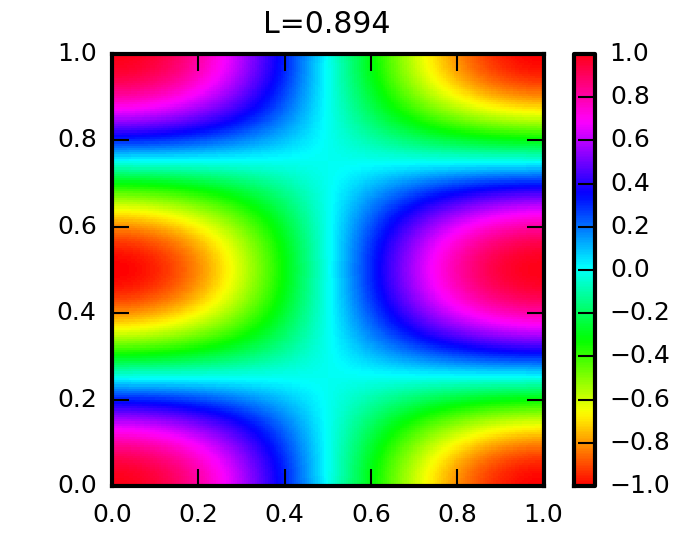
\includegraphics{figuras/modoanalitico_1_2.png}
  \end{subfigure}
  
  \caption{Modos de oscilaci\'on 3 y 6 obtenidos num\'ericamente para $h=1/25$ (primera columna) y mediante la soluci\'on anal\'itica para $(n,m)=(1,1)$ y $(n,m)=(1,2)$ (segunda columna)}
\end{figure}


  \subsection{Aplicaci\'on a la bah\'ia de Concepci\'on}

A partir de informaci\'on  de cartas n\'auticas del Servicio Hidrogr\'afico y Oce\'anico de la Armada de Chile \cite{shoa} se interpol\'o la topograf\'ia y batimetr\'ia correspondiente a la zona de la bah\'ia de Concepci\'on, y se utiliz\'o el software computacional AnuGA \cite{anuga} para generar la malla de elementos triangulares en el lugar de inter\'es, como se puede ver en la figura \ref{fig:bati-talcahuano}. La malla posee un total de 2697 nodos y 57600 tri\'angulos, y se impuso que el \'area de cada triangulo fuera menor que $57600m^2$. 

La condici\'on de borde por el lado que da hacia el oc\'eano no es trivial de implementar, y como una primera aproximaci\'on se simul\'o como un borde s\'olido, lo cual es consistente con el caso l\'imite en que las ondas quedan completamente atrapadas al interior. De esta forma, la bah\'ia completa se consider\'o como si estuviera cerrada por todos los bordes. 

Dadas estas definiciones, los seis primeros modos de oscilaci\'on y los per\'iodos asociados se encuentran representados en la figura \ref{fig:modos_talcahuano}.

\begin{figure}
  \centering
  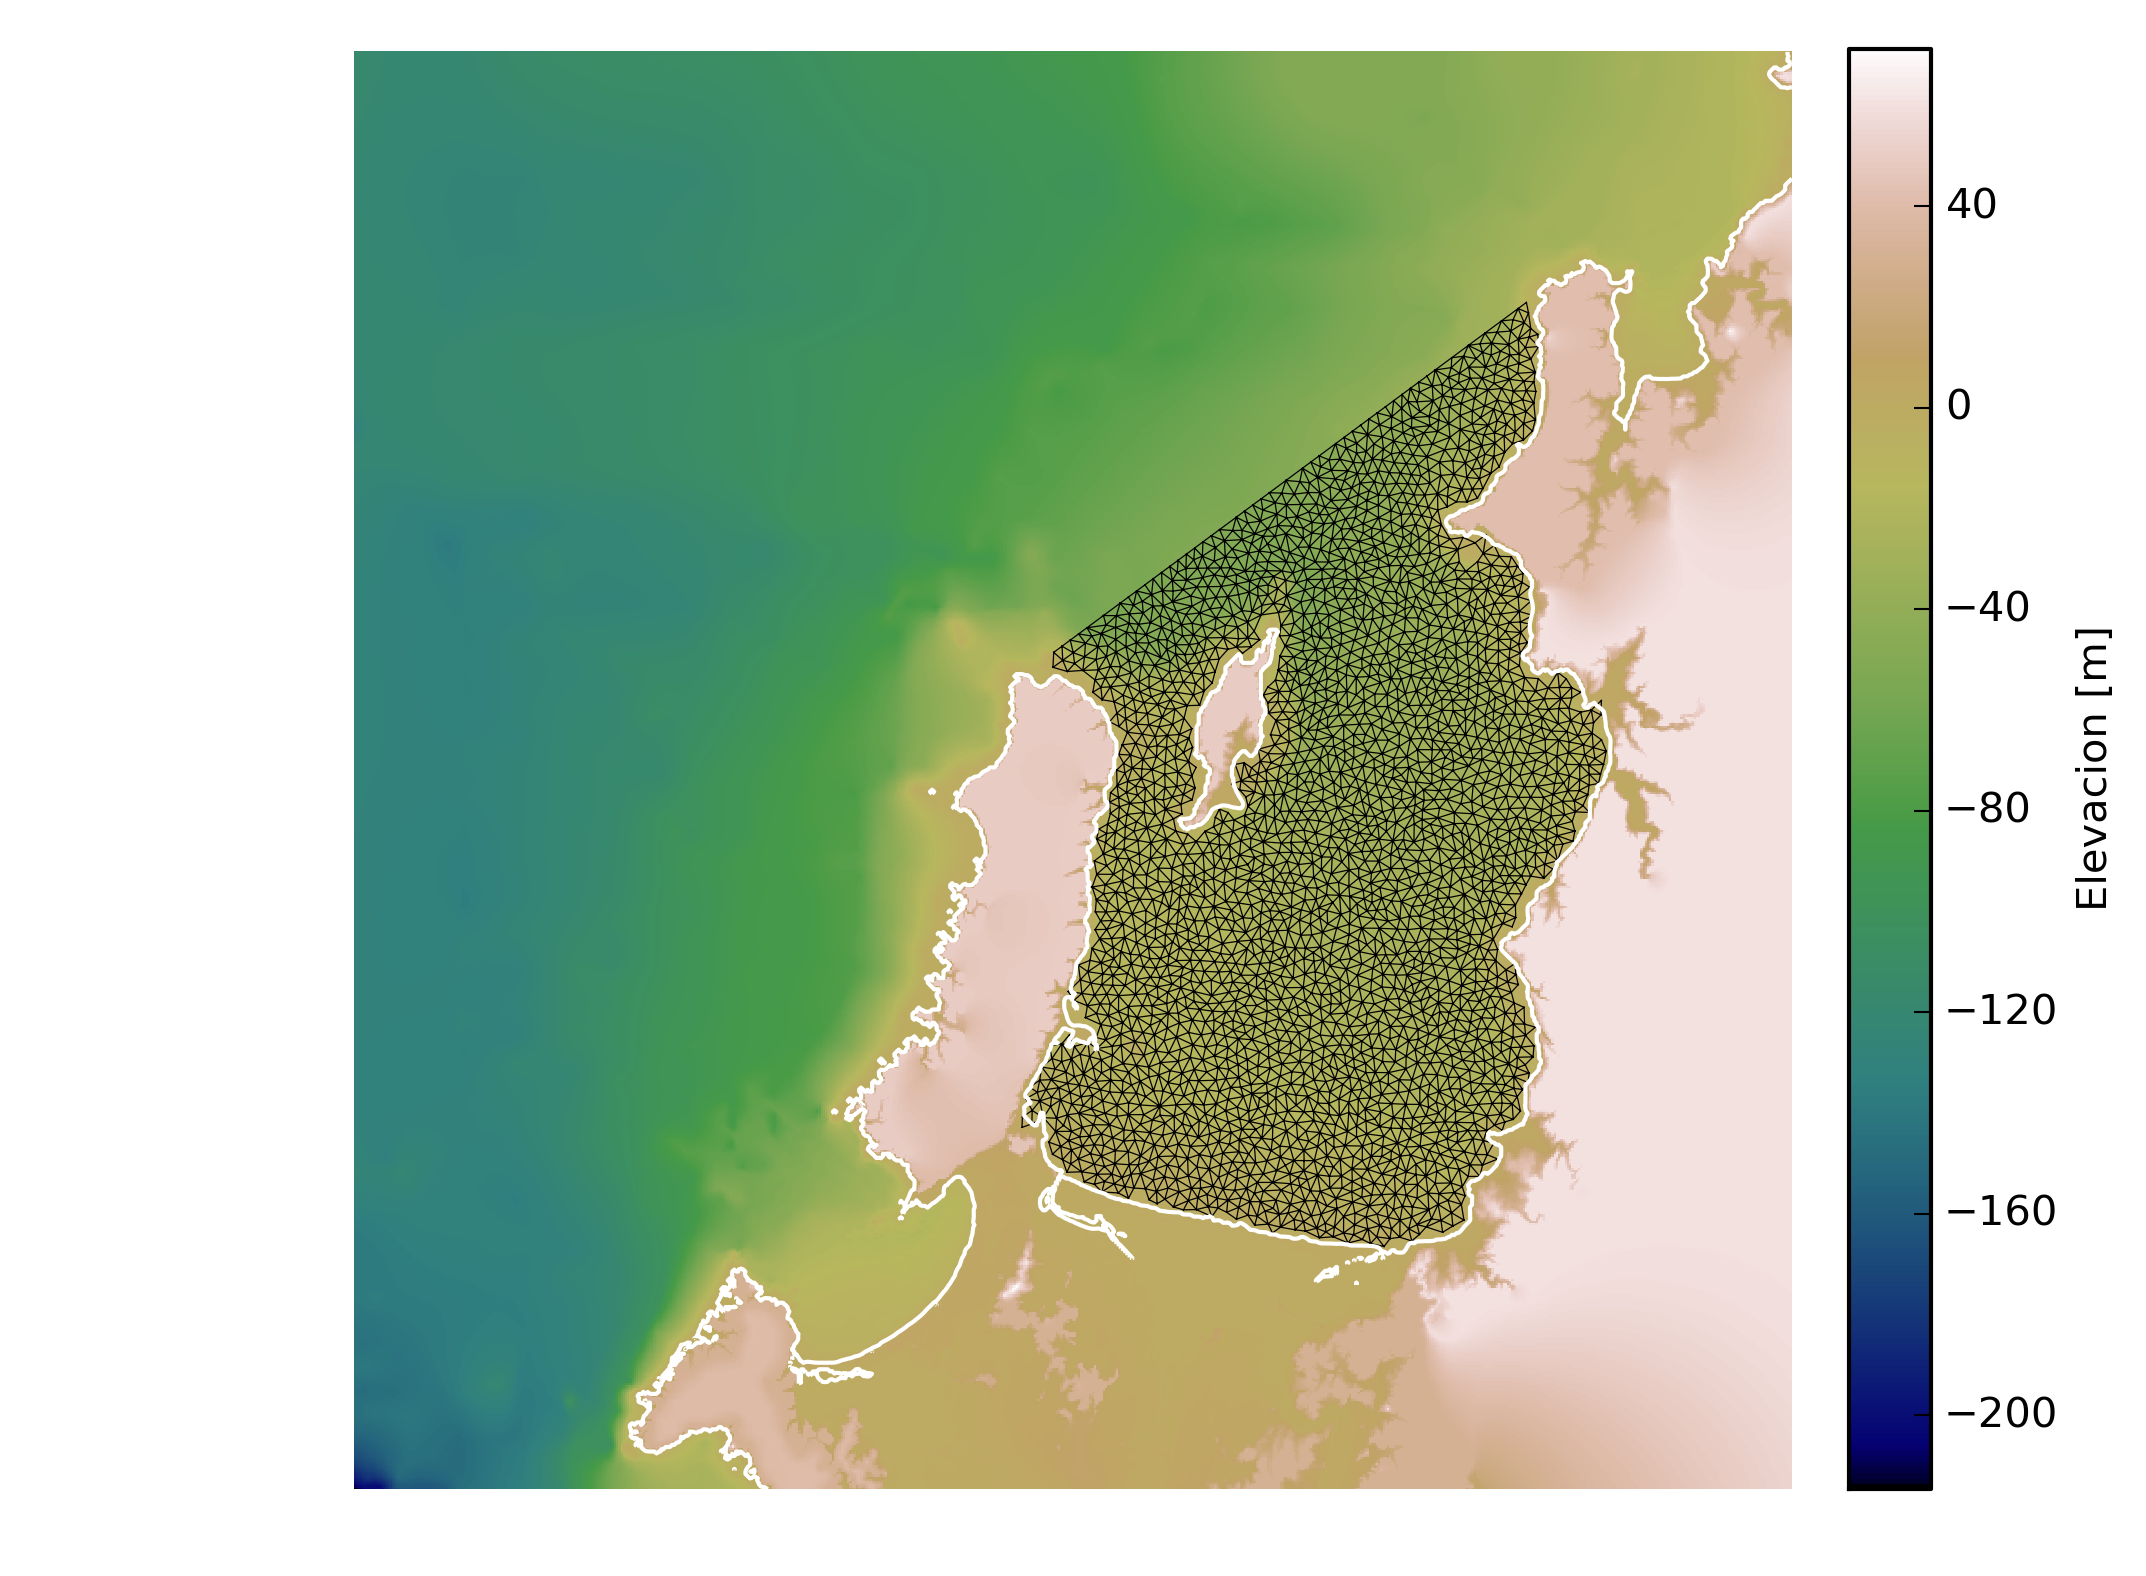
\includegraphics[width=15cm]{figuras/04bati+malla.png}
  \caption{ Batimetr\'ia y topograf\'ia de Talcahuano y malla triangular utilizada en la bah\'ia de Concepci\'on}  
  \label{fig:bati-talcahuano}
\end{figure}

\begin{figure}
  \begin{subfigure}{0.5\textwidth}
    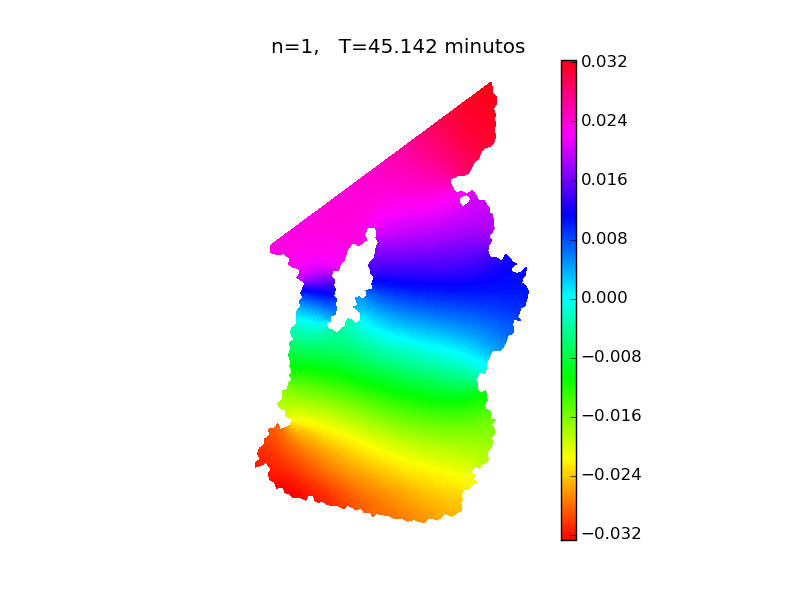
\includegraphics[width=\textwidth]{figuras/modos1.png}
  \end{subfigure}
  ~
  \begin{subfigure}{0.5\textwidth}
    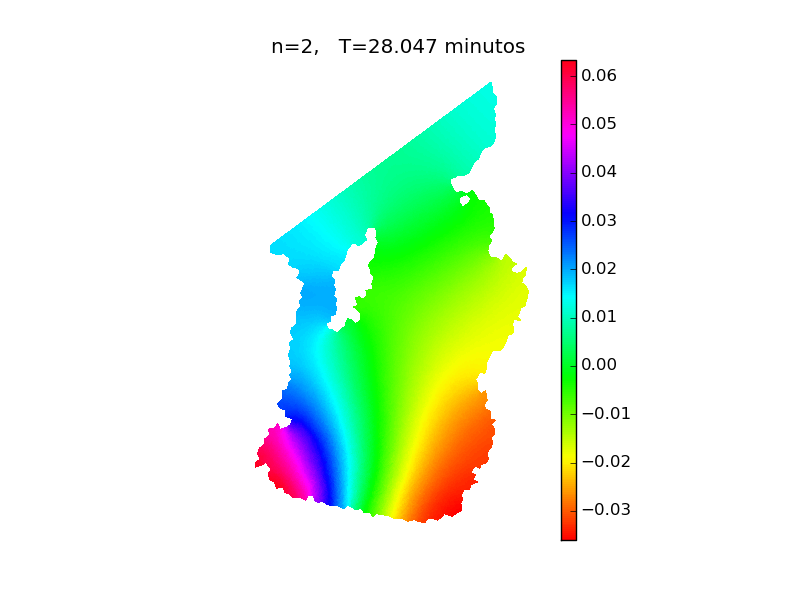
\includegraphics[width=\textwidth]{figuras/modos2.png}
  \end{subfigure}
  ~
  \begin{subfigure}{0.5\textwidth}
    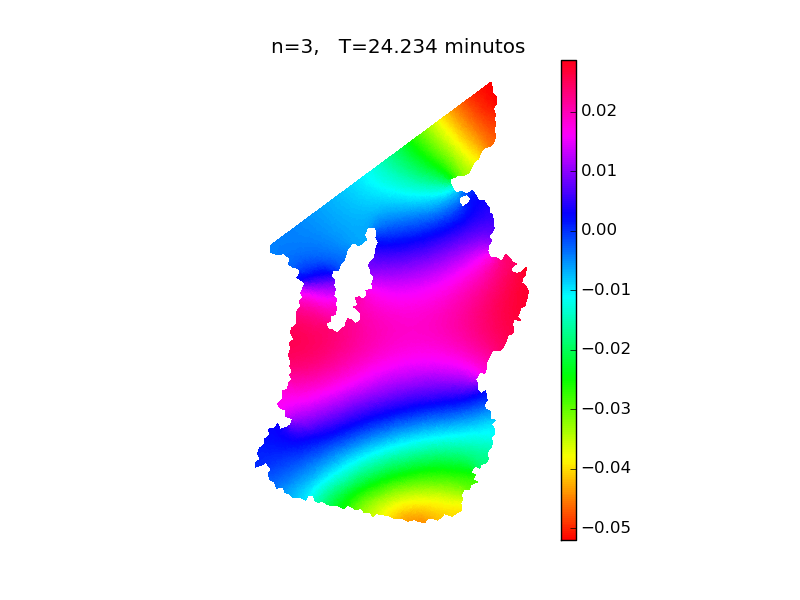
\includegraphics[width=\textwidth]{figuras/modos3.png}
  \end{subfigure}
  ~
  \begin{subfigure}{0.5\textwidth}
    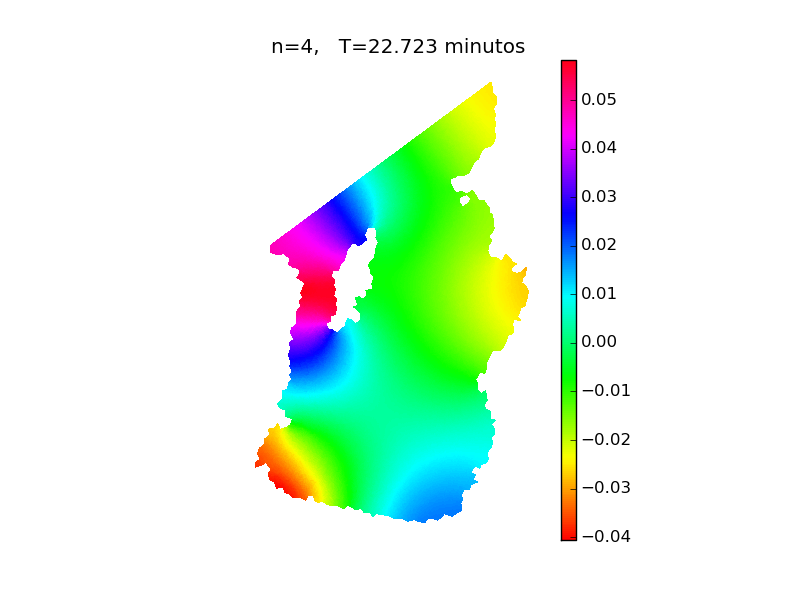
\includegraphics[width=\textwidth]{figuras/modos4.png}
  \end{subfigure}
  \\
  \begin{subfigure}{0.5\textwidth}
    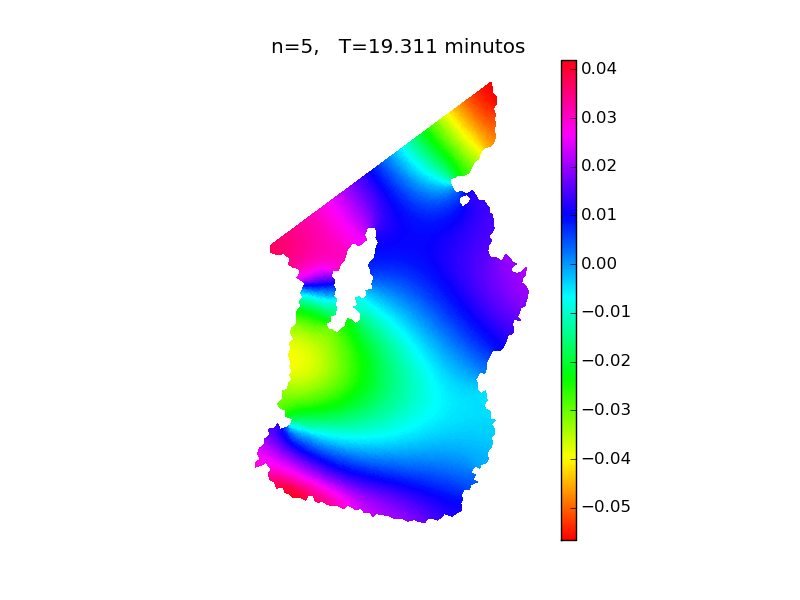
\includegraphics[width=\textwidth]{figuras/modos5.png}
  \end{subfigure}
  ~
  \begin{subfigure}{0.5\textwidth}
    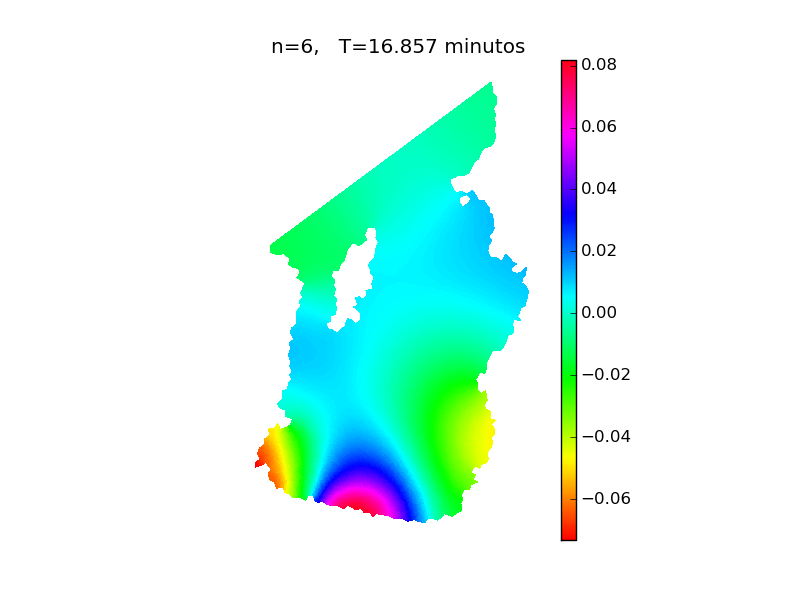
\includegraphics[width=\textwidth]{figuras/modos6.png}
  \end{subfigure}
  
  \caption{Primeros seis modos y per\'iodos de oscilaci\'on obtenidos para la configuraci\'on de la bah\'ia de Concepci\'on}
  \label{fig:modos_talcahuano}
\end{figure}
%   asfadsf
un resultado muy bac\'an
%En esta secci\'on usted debe presentar los resultados obtenidos de su investigaci\'on, en una secuencia l\'ogica. En esta secci\'on usted NO debe interpretar los resultados ni concluir algo a partir de estos. Sin embargo, si puede destacar algunos resultados importantes (por ejemplo, {\it es importante notar que el valor del estiramiento principal mayor alcanzan valores sobre 1.5, que corresponden a una deformaci\'on axial del 50 \%}) que ser\'an el punto de partida de sus conclusiones en la secci\'on de discusi\'on. Los gr\'aficos deben ser confeccionados con mucha atenci\'on, de manera de ser muy claros y no tener demasiada informaci\'on que dificulte leerlos. Sin embargo, sea elegante y eficiente, y no genere gr\'aficos que no reporten informaci\'on importante. No olvide agregar leyendas para las figuras (con el comando {\tt \textbackslash caption}) que ayuden la compresi\'on de estas (no repita informaci\'on en el texto principal). Para un ejemplo, vea la figura \ref{fig:tvconv}.



\section{Discusi\'on}
    Para el caso de la bah\'i rectangular se verifica lo mencionado en el \'ultimo p\'arrfo de la secci\'on \ref{subsec:ecuaciones}, dado que el menor de los valores propios calculados, en particular, siempre es igual a 0. Sin embargo, el m\'etodo num\'erico para obtener el vector propio asociado, implementado en la funci\'on \verb;numpy.linalg.eig;, falla, entregando un vector que no se asemeja al exacto. Tambi\'en se verifica la multiplicidad de valores propios con vectores propios diferentes, como los de la figura \ref{fig:multiplicidad}, o como se puede ver en la figura \ref{multiplicidad}, y que para este caso en particular obedece a las caracter\'isticas de simetr\'i de la bah\'ia, por ejemplo, pero que tambi\'en se pueden encontrar en otros casos como cuando $\sqrt{n^2+m^2}$ es un n\'umero natural (cuadrado perfecto). Sin embargo, todos los valores propios obtenidos num\'ericamente dieron valores no complejos, con lo cual se verifica lo expresado en la secci\'on \ref{subsec:ecuaciones}\cite{nica2011}. Adem\'as, en la figura \ref{multiplicidad} se observa que una mejor discretizaci\'on, adem\'as de permitir una mejor representaci\'on de los modos con longitud de onda largas, permite a\~nadir longitudes m\'as cortas a la colecci\'on de modos propios obtenidos por el m\'etodo.
  
  En la comparaci\'on entre la soluci\'on anal\'itica y la aproximaci\'on de Elementos Finitos se oberva que cualitativamente los vectores asociados a cada modo propio muestran notable similitud en t\'erminos de los nodos, antinodos y geometr\'ia general, lo cual se puede verificar, por ejemplo, en la figura \ref{fig:modos_numericovsanalitico}. En t\'erminos cuantitativos, la convergencia de los vectores y valores propios asociados a los primeros modos de oscilaci\'on puede tener orden 2 o superior, al medirlo experimentalmente usando la norma de $\mathcal{L}^2$ y de $\mathbb{R}$ respectivamente, como se ve en las  tablas \ref{tabla:EL} y \ref{tabla:Eu}.
  
%   \\
  
  En el caso de la bah\'ia de Concepci\'on, se verifica que los vectores propios obtenidos, mostrados en la figura \ref{fig:modos_talcahuano}, presentan forma similar a los que se encuentran en la literatura para estudios similares en puertos. Adem\'as se puede observar que los primeros vectores propios son, a grandes rasgos, similares a los de la bah\'ia rectangular, y caracterizados por tener el primero una linea nodal ($u=0$) en la direcci\'on $x$ y dos antinodos en los extremos Norte y Sur de la bah\'ia; el segundo una l\'inea nodal vertical; el tercero dos lineas nodales de orientaci\'on prominentemente horizontal; y el cuarto dos lineas nodales con orientaci\'on NorOeste - SurEste, pero que ya muestran una distorsi\'on m\'as dr\'astica que en los otros casos. 
  
  En particular, los resultados aqu\'i obtenidos par la distribuci\'on espacial de los vectores asociados a los modos propios, presentan, en forma cualitativa, similitud respecto a lo reportado en la literatura \cite{Belloti2012}, lo cual sugiere la validez de la implementaci\'on aqu\'i realizada. Adem\'as, al examinar la informaci\'on disponible en la literatura respecto al tsunami del 2010 \cite{Yamazaki2011}, se encuentra que el per\'iodo principal de oscilacion de \'este es del orden de $40$ minutos, y que corresponde al primer per\'iodo de oscilaci\'on aqu\'i obtenido. Una siguiente etapa de este trabajo incluir\'a la investigaci\'on de los fen\'omenos de resonancia que se pudieron haber observado en la bah\'i de Concepci\'on para el caso del tsunami del 2010.
  
  
%En esta secci\'on usted debe interpretar sus resultados presentados en la secci\'on anterior, y compararlos/contrastarlos con resultados conocidos previamente en otros art\'iculos o libros. Lo anterior le permitir\'a generar conclusiones a partir de la interpretaci\'on de sus resultados. Sea claro en los pasos de su razonamiento que lo llevan a sus conclusiones. La secci\'on de discusi\'on debe responder las preguntas o verificar las hip\'otesis planteadas en la secci\'on de {\it introducci\'on}. Es recomendable tambi\'en incluir en la discusi\'on cuales son las limitantes de su investigaci\'on, y c\'omo pueden afectar los resultados y conclusiones obtenidas. Finalmente, es recomendable incluir posibles ideas \'o proyectos futuros que nacen a ra\'iz del trabajo de investigaci\'on presentado en el art\'iculo.


\begin{thebibliography}{10}

\bibitem{nica2011}
  M. Nica. Eigenvalues and Eigenfunctions of the Laplacian. \emph{The Waterloo Mathematics Review} 2011; {\bf 1}, No.2, 23--34.
\bibitem{hughes2000}
  T.J.R. Hughes, \emph{The finite element method: Linear static and dynamic finite element analysis}. Dover Publications, 2000.
  
\bibitem{zienkiewicz2006}
  O.C. Zienkiewicz, R.L. Taylor, J.Z. Zhu, \emph{The finite element method: Its basis and fundamentals}. Sixth edition, Butterworth-Heinemann, 2006.  

\bibitem{riceweb} {\tt http://www.ruf.rice.edu/~bioslabs/tools/report/reportform.html }

\bibitem{goktepekuhl2009}
	S. G\"{o}ktepe and E. Kuhl.Computational modeling of cardiac electrophysiology: A novel finite element approach. \emph{International Journal for Numerical Methods in Engineering} 2009; {\bf 79}, 156--178.
	
\bibitem{Kowalik1993}
	Z. Kowalik and T.S. Murty. \emph{Numerical modeling of ocean dynamics. Advanced Series.on Ocean Engineering, vol. 5. }World Scientific, Singapore. 1993; 
	
\bibitem{Mei2005}
	C. Mei, M. Stiassnie and D. Yue \emph{Theory and applicaction of suface ocean Waves, vol. 5. }World Scientific, Singapore. 2005; 

\bibitem{Diaz2006web} {\tt http://www.tdx.cat/bitstream/handle/10803/10618/}

\bibitem{Cyper2012web} {\tt http://ciperchile.cl/2012/01/18/tsunami-paso-a-paso-los-escandalosos} {\tt-errores-y-omisiones-del-shoa-y-la-onemi/
}

\bibitem{Belloti2012}
	G. Belloti, R. Briganti, G. M. Beltrami, L. Franco. Modal analysis of semi-enclosed basins. \emph{Coastal Engineering} 2012; {\bf 64}, 16--25.

\bibitem{Rabino2009}
	A.B. Rabinovich. Seiches and harbor oscillations. \emph{Handbook of coastal and ocean engineering. World Scientific Publ} 2009; {\bf 64}, 193--236.

\bibitem{Yamazaki2011}
	Y. Yamazaki and K. F. Cheung. Shelf resonance and impact of near-field tsunami generated by the 2010 Chile earthquake. {\it Geophysical Research Letters}. Vol 38. (2011)

\bibitem{anuga}
	O. Nielsen, S. Roberts, D. Gray, A. McPherson and A. Hitchman. Hydrodynamic modelling of coastal inundation. URL: \verb; http://www.ga.gov.au/webtemp/image_cache/GA7981.pdf;
\bibitem{shoa}
      Servicio Hidrogr\'afico y Oceanogr\'fico de la Armada de Chile. \verb;http://www.shoa.cl;
\bibitem{toro}
      E. Toro. Shock capturing methods for free surface shallow flows. John Wiley, 2001.
\end{thebibliography}

% \appendix
% 
% \section{Sobre los ap\'endices}
% 	Los ap\'endices contienen informaci\'on que no es de car\'acter esencial para entender el art\'iculo. Muchas derivaciones de ecuaciones, demostraciones de teoremas (con la salvedad de art\'iculos en revistas de matem\'atica), tablas de datos, etc., son inclu\'idas en el ap\'endice.
% 	
% \section{Sobre la evaluaci\'on del art\'iculo final}
% 	El art\'iculo final ser\'a evaluado tanto en los aspectos acad\'emicos (calidad de los resultados obtenidos) como en aspectos de presentaci\'on y redacci\'on. En particular, se considerar\'a en la evaluaci\'on la redacci\'on, diagramaci\'on, ortograf\'ia, correcta referenciaci\'on (incluir las citas y bibliograf\'ia), gr\'aficos y figuras, entre otros.
% 



\end{document}
